\chapter{PLANTEAMIENTO DEL PROBLEMA}
En el presente capítulo se mostrará el cáncer como una enfermedad mortal presente en todo el mundo. (Se mejorará cuando se concluya el capítulo).
\section{Descripción de la Realidad Problemática}

El cáncer es una de las enfermedades más mortales que puede manifestarse en cualquier etapa de la vida de una persona, convirtiéndose en un problema de salud pública a nivel mundial. Según datos de la Organización Mundial de la Salud (OMS) y la Sociedad Americana de Cáncer, el riesgo global de desarrollar cáncer se estima en 20.2\% para individuos de 0 a 74 años, y cerca de 10 millones de defunciones fueron atribuidas a esta enfermedad en 2020. Se ha determinado que uno de cada dos hombres y una de cada tres mujeres será diagnosticado con cáncer en algún momento de su vida. Además, cerca de 400 000 niños contraen cáncer cada año.

A nivel global, los tres tipos de cáncer más comunes fueron el de mama (2.26 millones de casos), pulmón (2.21 millones de casos) y colorrectal (1.93 millones de casos). Por otro lado, los más mortales fueron el de pulmón (1.8 millones de defunciones), colorrectal (916 000 defunciones) y hepático (830 000 defunciones). La carga de la enfermedad asociada al cáncer es muy alta, siendo responsable de 2668.475 millones de años de vida ajustados por discapacidad, lo que lo convierte en una de las enfermedades con mayor impacto a nivel mundial.

En América Latina y el Caribe, la situación es igualmente crítica. De acuerdo con los datos de GLOBOCAN 2022, se reportaron aproximadamente 1.55 millones de nuevos casos de cáncer en la región durante ese año, con 700 mil muertes, lo que equivale a una tasa de incidencia de 186.0 por cada 100 mil habitantes y una tasa de mortalidad de 233.1 por cada 100 mil habitantes. Se estima que la carga de la enfermedad continuará aumentando, y para el año 2040 la incidencia del cáncer en la región podría incrementarse en un 69\%. A pesar de los avances en la lucha contra el cáncer en América Latina y el Caribe, persisten problemas críticos como los sistemas de salud fragmentados, la inequidad en el acceso a servicios médicos, la falta de registros adecuados y el acceso limitado a datos. Todo esto hace urgente mejorar el control del cáncer en la región.

En la Figura \ref{1:fig} y Figura \ref{2:fig} se observa la distribución del cáncer a nivel global, tanto en incidencia como en mortalidad, recolectados por GLOBOCAN 2022.%\medskip

\begin{figure}[ht]
    \centering
    % Primera figura
    \begin{minipage}[b]{0.48\textwidth}
        \centering
        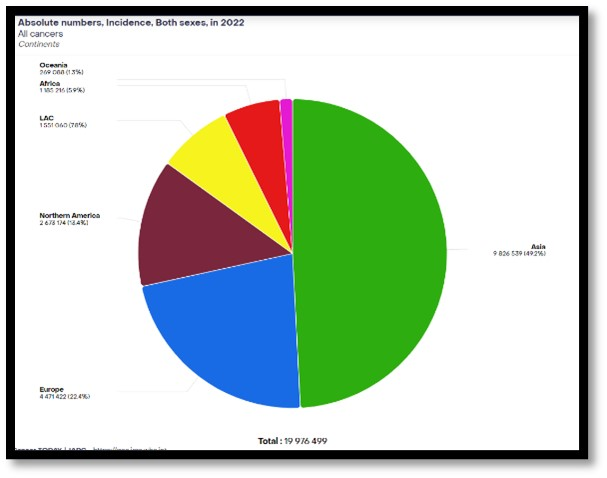
\includegraphics[width=\textwidth]{1/figures/Incidencias.jpg}
        \caption{Números absolutos, Incidencia, Ambos sexos, en 2022 (Todos los cánceres, todos los continentes). Fuente:\cite{iarc}}
        \label{1:fig}
    \end{minipage}
    \hfill
    % Segunda figura
    \begin{minipage}[b]{0.48\textwidth}
        \centering
        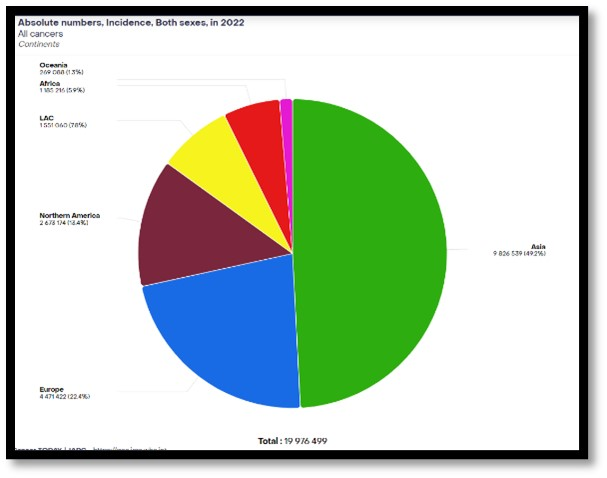
\includegraphics[width=\textwidth]{1/figures/Incidencias.jpg}
        \caption{Números absolutos, Mortalidad, Ambos sexos, en 2022 (Todos los cánceres, todos los continentes). Fuente:\cite{iarc}}
        \label{2:fig}
    \end{minipage}
\end{figure}

Considerando el impacto global del cáncer, es importante enfocarnos en el contexto nacional. En Perú, esta enfermedad representa una de las principales causas de mortalidad y ha sido declarada una prioridad por el Ministerio de Salud (Minsa) y el Seguro Social de Salud (EsSalud). La Agencia Internacional para la Investigación en Cáncer (IARC) estimó para 2020 un total de 69 869 nuevos casos de cáncer en Perú y 34 976 defunciones por cáncer.

Mediante la información recolectada por el Centro Nacional de Epidemiología, Prevención y Control de Enfermedades, podemos observar la tendencia y distribución de casos registrados de pacientes con cáncer en las Figuras N°\ref{3:fig} y N°\ref{4:fig}

\begin{figure}[ht]
	\centering
	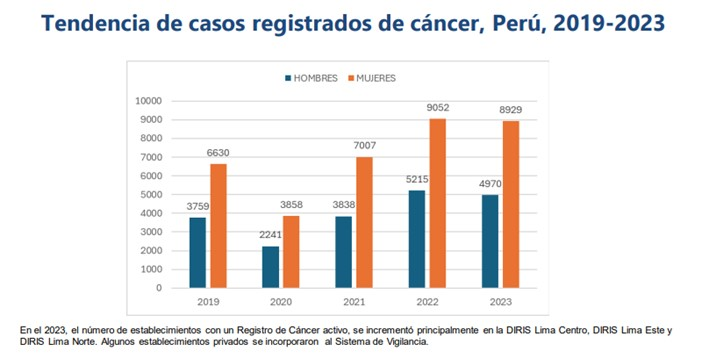
\includegraphics[width=1.1\textwidth]{1/figures/Tendencia.jpg}
	\caption{Tendencia de casos registrados de cáncer, Perú, 2019-2023. Fuente: \cite{cdc2023cancer}}
	\label{3:fig}
\end{figure}

\begin{figure}[h!]
	\centering
	\includegraphics[width=1.1\textwidth]{1/figures/Distribución.jpg}
	\caption{Distribución de casos registrados de cáncer por edad y sexo, Perú, 2023. Fuente: \cite{cdc2023cancer}}
	\label{4:fig}
\end{figure}

Se obtuvo que una proporción significativa de casos le pertenece al cáncer de mama. Este tipo de cáncer afecta a miles de mujeres cada año, y su diagnóstico en etapas avanzadas aumenta la complejidad del tratamiento y reduce las posibilidades de supervivencia.
El cáncer de mama es el tipo de cáncer más frecuente en mujeres peruanas, y sus efectos son devastadores tanto física como emocionalmente. Esta enfermedad no solo amenaza la vida de las pacientes, sino que también conlleva profundas repercusiones en su bienestar emocional, social y económico. Las mujeres con cáncer de mama pueden experimentar síntomas como la aparición de un bulto en el seno, cambios en la forma o tamaño del seno, secreción del pezón, y dolor en las mamas. Sin embargo, muchas veces, los síntomas no son evidentes en las primeras etapas, lo que dificulta la detección temprana y aumenta el riesgo de que la enfermedad avance a estadios más peligrosos.
Cuando el cáncer de mama se diagnostica en etapas avanzadas, las consecuencias son mucho más graves. El tratamiento suele ser más invasivo y costoso, e implica quimioterapia, radioterapia o cirugías complejas como la mastectomía, que afecta significativamente la imagen corporal de la mujer. Además del impacto físico, las pacientes pueden sufrir una fuerte carga emocional, ya que el tratamiento conlleva efectos secundarios como pérdida de cabello, fatiga extrema, náuseas y un estado de vulnerabilidad emocional que puede llevar a la ansiedad y la depresión. La enfermedad no solo afecta a la paciente, sino también a su entorno familiar, social y laboral, generando una carga financiera y emocional considerable.
El cáncer de mama no tratado a tiempo puede diseminarse a otras partes del cuerpo, como los huesos, los pulmones o el hígado, lo que se conoce como metástasis, lo que disminuye drásticamente las probabilidades de supervivencia. En Perú, la situación es especialmente preocupante debido a la alta tasa de diagnósticos en etapas avanzadas. La mayoría de las mujeres que desarrollan cáncer de mama provienen de áreas rurales o poblaciones vulnerables, donde el acceso a servicios médicos es limitado, y la falta de información sobre la autoexploración y los chequeos médicos regulares es alarmante. Esta distribución se puede observar en la Figura N°\ref{5:fig}.
\begin{figure}[ht]
	\centering
	\includegraphics[width=1.1\textwidth]{1/figures/Estadificación.jpg}
	\caption{Estadificación del cáncer en los casos registrados, Perú, 2023. Fuente: \cite{cdc2023cancer}}
	\label{5:fig}
\end{figure}
\vspace{0.5 cm}

Donde en el país los costos de tratamiento son altos pueden rondar entre los 200 000 soles a los 450 000 soles como mínimo (Aproximadamente pueden variar) que pueden incluir gastos en consultas médicas, exámenes de laboratorio, exámenes por imágenes, radioterapias, quimioterapias entre otros. Podemos darnos cuenta de esto mirando el tarifario por ejemplo del instituto nacional de enfermedades de neoplásicas en la figura N°\ref{6:fig}, solo para quimioterapia rondan entre los 37 soles a 595 soles teniendo en cuenta la eficacia y la rapidez de la atención, esto solo es la administración ya que los medicamentos administrados es otro precio a parte que incrementan el precio de la sesión.

\begin{figure}[ht]
	\centering
	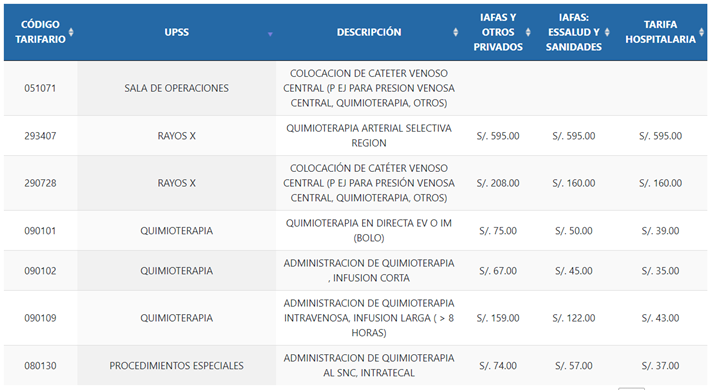
\includegraphics[width=1.1\textwidth]{1/figures/Tarifario.png}
	\caption{Tarifario- Quimioterapia. Fuente: \cite{inenTarifario}}
	\label{6:fig}
\end{figure}
\vspace{0.5 cm}

Sabiendo esto para un peruano seria vital tener un seguro oncológico, por el lado privado tendríamos a Oncosalud como ejemplo que brindan planes de cobertura con tarifas mensuales que incluyen gastos en medicamentos, tratamientos, citas médicas, entre otros, cabe resaltar que al optar por esta opción se debe tener en cuenta cuanto cubre y que cosas no.

Por el lado publico es un poco más complicado, teniendo que el Perú es un país donde desborda el trabajo informal y población de escasos recursos tanto en zona urbana y rural donde una gran cantidad de la población no con cuenta con seguro integral de Salud (SIS) o seguro social de salud (EsSalud), se puede apreciar esto en la figura N°\ref{7:fig}.

\begin{figure}[ht]
	\centering
	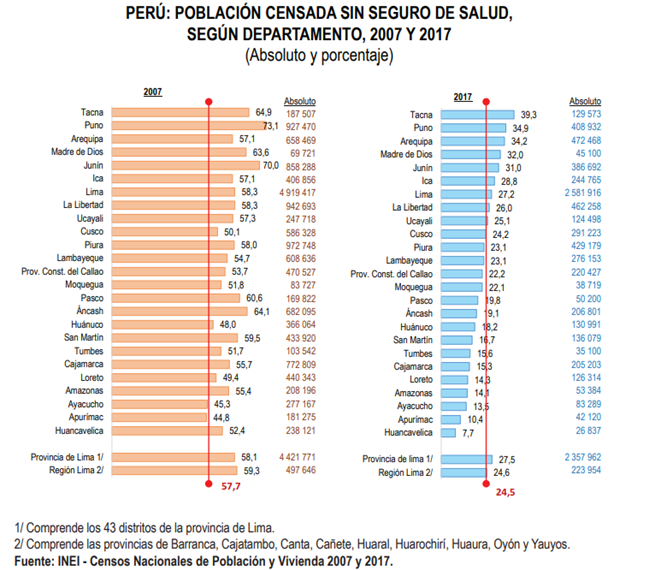
\includegraphics[width=1.1\textwidth]{1/figures/SINSEGURO.png}
	\caption{Población censada sin seguro de salud, según departamento, 2007 y 2017. Fuente: \cite{inei2018poblacion}}
	\label{7:fig}
\end{figure}

Sin embargo, en la población hay una gran tasa de desinformación y poco interés sobre el cáncer. Según la encuesta de Oncosalud junto a Ipsos Perú, se determinó que hombres y mujeres de 18 a 65 años no se sienten protegidos contra el cáncer y solo un 34\% de personas se sienten listas para enfrentar esta enfermedad a nivel de acceso al tratamiento y económico. Se obtuvo también que más de la mitad de los peruanos nunca se ha realizado un chequeo oncológico esta alta cifra se debe a la falta de información y al miedo de enfrentar la enfermedad.
Considerando todos estos factores, es importante señalar que el sistema de salud pública en Perú enfrenta deficiencias significativas. A pesar de que existen seguros públicos, no son suficientes para cubrir las necesidades de los pacientes debido a las largas colas, la escasez de medicamentos, la mala infraestructura, entre otros problemas que impiden una atención adecuada para enfrentar esta enfermedad. Además, una gran parte de la población vive en condiciones de pobreza o en zonas rurales donde el acceso a la información y a los servicios médicos es extremadamente limitado, lo que agrava la carga tanto para los pacientes como para sus familias. Esto se traduce en la acumulación de informes médicos, medicamentos, efectos secundarios, y otros factores que afectan gravemente la salud mental, un componente esencial para el bienestar general.
Si bien la medicina a avanzado junto con la tecnología haciendo un poco más fácil el tratamiento y la detección de esta enfermedad, se centra en eso, en decirle al paciente que tiene la enfermedad y ya. Y si tienes el dinero suficiente puedes tener todos los recursos para poder luchar contra la enfermedad, pero por el otro lado si no lo tienes estas condenado a morir.
Dada la magnitud de este desafío, es imperativo buscar soluciones innovadoras que puedan mitigar estos impactos adversos, especialmente en lugares donde el acceso a la información y a los servicios médicos es limitado. Aquí es donde las aplicaciones móviles entran en juego como un recurso vital. Según Okolo et al. (2024), que revisa el rol de las aplicaciones móviles en mejorar el compromiso del paciente y los resultados de salud, estas herramientas tecnológicas ofrecen un medio efectivo para gestionar la enfermedad de manera más eficiente. Las aplicaciones móviles no solo pueden facilitar el monitoreo constante de los signos vitales de los pacientes, sino que también permiten un acceso más fácil a información vital, mejorando la comunicación entre pacientes y proveedores de salud, y ofreciendo educación sobre la enfermedad que puede ser crucial para la detección temprana y la gestión efectiva del cáncer.
Aprovechando la tecnología móvil, los pacientes pueden superar las barreras geográficas y económicas que a menudo complican el acceso a tratamientos adecuados. Las aplicaciones pueden guiar a los usuarios en el proceso de autoexaminación, recordarles sus citas médicas y ciclos de medicación, y proporcionar información valiosa sobre los efectos secundarios y el manejo de la enfermedad. Esta interacción continua y accesible ayuda a reducir las colas en los hospitales, minimiza la escasez de medicamentos al permitir un mejor planeamiento y seguimiento, y puede mejorar significativamente la infraestructura de salud al reducir la carga sobre los recursos físicos.
En resumen, frente a un panorama tan desafiante como el del cáncer en Perú y en el mundo, es esencial integrar y aprovechar las tecnologías móviles para mejorar la atención del cáncer. No solo se trata de diagnosticar y tratar, sino de ofrecer una plataforma continua de apoyo y manejo que pueda hacer una diferencia significativa en la vida de los pacientes y sus familias, mejorando su calidad de vida y posiblemente sus tasas de supervivencia. Las aplicaciones móviles ofrecen una promesa tangible en esta lucha, demostrando ser no solo una necesidad sino una solución viable en el manejo moderno del cáncer.





\section{Formulación del Problema}

Habiendo presentado anteriormente el problema del cáncer tanto en el Perú y resto del mundo, podemos decir que la tecnología puede ayudar a los pacientes de cáncer, utilizando como herramienta algo que todos tienen un teléfono móvil, se presenta a continuación la formulación del problema central y los problemas específicos.

\subsection{Problema General}

\begin{itemize}
	\item \textit{PG} : ¿De qué manera una aplicación móvil mediante el uso de inteligencia artificial generativa puede contribuir al control, monitoreo integral y educación de los pacientes con cáncer de mama?
 
\end{itemize}

 \subsection{Problemas específicos}
 \begin{itemize}
         \item \textit{PE 1} : ¿Qué base de datos se deben usar para entrenar el modelo de inteligencia artificial para ofrecer respuestas optimas?
         \item \textit{PE 2} : ¿De qué manera una aplicación móvil puede proporcionar soporte emocional a los pacientes oncológicos?
         \item \textit{PE 3} : ¿Qué funcionalidades de una aplicación móvil son esenciales para el monitoreo de signos vitales en pacientes con cáncer?
          \item \textit{PE 4} : ¿Cómo puede una aplicación móvil proporcionar información personalizada y actualizada sobre el cáncer de mama utilizando IA generativa?
          \item \textit{PE 5} : ¿Qué modelo de IA generativa se va a implementar para que las funciones de la aplicación móvil funcionen correctamente?
          

\end{itemize}

\section{Objetivos de la Investigación}
A continuación, se presentarán el objetivo central y específicos de esta investigación.

\subsection{Objetivo General}
\begin{itemize}
	\item \textit{OG} : Desarrollar una aplicación móvil basada en Inteligencia Artificial generativa para el monitoreo integral y el control de pacientes con cáncer, que mejore la adherencia al tratamiento, el seguimiento de signos vitales, el soporte emocional y conocimiento sobre la enfermedad.
 
\end{itemize}

 \subsection{Objetivos específicos}
 \begin{itemize}
         \item \textit{OE 1} : Identificar las bases de datos especializadas que se pueden integrar para entrenar el modelo de IA generativa de la aplicación móvil.
         \item \textit{OE 2} : Implementar un sistema de IA generativa que proporcione soporte emocional personalizado en función del estado anímico del paciente.
         \item \textit{OE 3} : Desarrollar e integrar un sistema de monitoreo de signos vitales en tiempo real que notifique a los pacientes sobre anomalías.
         \item \textit{OE 4} : Desarrollar una funcionalidad que permita a los pacientes recibir información personalizada y actualizada sobre su condición.
         \item \textit{OE 5} : Seleccionar y optimizar el modelo de IA generativa más adecuado para integrar todas las funciones de la aplicación móvil de manera eficiente.
\end{itemize}
\section{Hipótesis General}
En este presente trabajo de investigación, se pretende comprobar que la utilización de una aplicación móvil mejorar en el soporte integral de un paciente con cáncer de mama. La hipótesis general del presente proyecto de investigación es la siguiente.
\subsection{Hipótesis general }
\begin{itemize}
	\item \textit{HG} : El desarrollo de una aplicación móvil que emplea Inteligencia Artificial generativa mejorará significativamente el monitoreo integral, el control y la educación de pacientes con cáncer de mama.
 
\end{itemize}

\subsection{Hipótesis específicos}
 \begin{itemize}
         \item \textit{HE 1} : El desarrollo de una aplicación móvil que emplea Inteligencia Artificial generativa mejorará significativamente el soporte integral y la educación de pacientes con cáncer de mama.
         \item \textit{HE 2} : La implementación de un sistema de soporte emocional automatizado mejorará el bienestar emocional de los pacientes, reduciendo su ansiedad y mejorando su calidad de vida.
         \item \textit{HE 3} : La integración de un sistema de monitoreo de signos vitales basado en IA reducirá las complicaciones relacionadas con la falta de detección temprana de problemas.
         \item \textit{HE 4} : La implementación de un sistema que proporcione información personalizada mejorará el conocimiento del paciente sobre su enfermedad y su tratamiento.
         \item \textit{HE 5} : La implementación de un modelo de IA generativa optimizado permitirá que todas las funciones de la aplicación móvil (soporte emocional, monitoreo de signos vitales, información personalizada) funcionen de manera eficiente y precisa.
         

\end{itemize}

\section{Justificación de la Investigación}
A continuación, se presentarán la justificación teórica, práctica y metodológica para la elaboración de este proyecto.
\subsection{Justificación Teórica}
El cáncer de mama representa una de las principales causas de mortalidad a nivel mundial, lo que subraya la urgente necesidad de mejorar el soporte integral a los pacientes, abarcando tanto el monitoreo de su salud como el apoyo emocional y psicológico durante su tratamiento \parencite{pascucci2021}. La literatura científica reciente ha puesto de manifiesto la importancia crítica de desarrollar soluciones tecnológicas innovadoras que permitan a los pacientes acceder de manera rápida y efectiva a información personalizada sobre su condición, así como facilitar un monitoreo continuo y preciso de su salud \parencite{okolo2024}.

Los avances significativos en el campo de la inteligencia artificial, particularmente en el área de la IA generativa, ofrecen oportunidades sin precedentes para crear herramientas de atención médica altamente personalizadas. Esto se evidencia en la aplicación exitosa de modelos de lenguaje natural y algoritmos sofisticados de procesamiento de datos médicos en diversas áreas de la oncología \parencite{ce2024}. Estos modelos avanzados no solo permiten ofrecer recomendaciones y respuestas en tiempo real, sino que también tienen el potencial de asistir en la detección temprana de complicaciones relacionadas con el cáncer de mama, como cambios sutiles en los signos vitales o la aparición de lesiones cutáneas que podrían pasar desapercibidas \parencite{naeem2022}.

En paralelo, la aplicación de tecnologías móviles en el ámbito de la salud ha demostrado ser un medio excepcionalmente eficaz para mejorar la adherencia de los pacientes a sus tratamientos y promover la autogestión efectiva de sus condiciones crónicas \parencite{masciantonio2017}. Las aplicaciones móviles de salud han sido utilizadas con éxito para monitorear parámetros críticos, mejorar la comunicación bidireccional entre pacientes y médicos, y ofrecer un apoyo emocional continuo, aspectos que son particularmente cruciales para pacientes oncológicos que experimentan altos niveles de estrés y ansiedad durante su tratamiento \parencite{leung2022}.

En este contexto, el desarrollo de una aplicación móvil que integre de manera innovadora la IA generativa con el monitoreo exhaustivo de la salud busca atender de manera holística las múltiples y complejas necesidades de los pacientes con cáncer de mama. Al incorporar funcionalidades avanzadas como la detección precisa de signos vitales, un soporte emocional adaptativo, y la posibilidad de acceder a recomendaciones personalizadas sobre nutrición y manejo del tratamiento, la aplicación no solo empodera a los pacientes, sino que también tiene el potencial de mejorar significativamente sus resultados de salud a largo plazo \parencite{beltran2023}.

Además, es importante destacar el potencial de esta tecnología para abordar las disparidades en el acceso a la atención médica, especialmente en regiones con recursos limitados o en áreas rurales donde el acceso a especialistas oncológicos puede ser restringido \parencite{smith2023}. La aplicación móvil propuesta podría servir como un puente vital, proporcionando información crucial y monitoreo continuo a pacientes que de otra manera podrían tener un acceso limitado a estos recursos.

En conclusión, esta tesis se justifica en la creciente y apremiante necesidad de ofrecer a los pacientes con cáncer de mama un sistema integral y tecnológicamente avanzado de soporte a través de la convergencia de tecnologías innovadoras como la IA generativa y las aplicaciones móviles de salud. La implementación de una aplicación móvil de estas características permite abordar de manera efectiva los múltiples desafíos que enfrentan los pacientes, mejorando significativamente la accesibilidad a información personalizada, asegurando la continuidad en el monitoreo de su estado de salud, y elevando la calidad del soporte emocional que reciben. Estos elementos son fundamentales para el manejo efectivo y humanizado del cáncer de mama en la era digital.


\subsection{Justificación Práctica}
El cáncer de mama no solo es una de las principales causas de mortalidad en el mundo, sino que también representa un desafío significativo en el monitoreo continuo y en el soporte emocional para los pacientes. Las barreras de acceso a atención especializada y las limitaciones en el seguimiento personalizado de los tratamientos son problemas comunes en los sistemas de salud, especialmente en países de bajos y medianos ingresos \parencite{pascucci2021}. En este contexto, el desarrollo de una aplicación móvil que integre múltiples funcionalidades para el soporte de pacientes con cáncer de mama ofrece una solución práctica y viable.

El uso de aplicaciones móviles en el sector salud ha demostrado ser una herramienta eficiente para la autogestión de enfermedades crónicas, facilitando la adherencia a tratamientos y mejorando la comunicación entre pacientes y médicos \parencite{okolo2024}. La incorporación de IA generativa en esta aplicación permitirá generar respuestas personalizadas en tiempo real y ofrecer recomendaciones basadas en el análisis continuo de los datos de salud de los pacientes, como sus signos vitales y reportes de síntomas \parencite{ce2024}.

En la práctica, esta aplicación se presenta como una herramienta accesible para pacientes con cáncer de mama que enfrentan barreras geográficas o económicas para acceder a atención médica regular \parencite{leung2022}. Mediante el uso de smartphones, la aplicación permitirá el monitoreo remoto y la detección temprana de complicaciones, tales como cambios en los signos vitales o la aparición de nuevas lesiones en la piel. Esto reducirá la necesidad de visitas presenciales y permitirá una intervención médica más oportuna y eficiente \parencite{masciantonio2017}. Además, se ofrecerán recomendaciones personalizadas sobre nutrición, soporte emocional y manejo de tratamientos, lo que aumentará el compromiso de los pacientes y mejorará sus resultados de salud a largo plazo \parencite{beltran2023}.

El enfoque práctico de esta tesis radica en ofrecer una solución tecnológica integrada que no solo ayuda a los pacientes, sino que también reduce la carga en los sistemas de salud al permitir un seguimiento más eficiente y continuo sin depender completamente de consultas médicas presenciales \parencite{pascucci2021}. Los médicos podrán tomar decisiones más informadas y rápidas gracias a la disponibilidad de datos en tiempo real, mejorando la calidad del tratamiento y el bienestar del paciente. La aplicación es de fácil implementación y escalable, lo que significa que podría adaptarse para otros tipos de cáncer o enfermedades crónicas, generando un impacto positivo en la atención de la salud a nivel global.

En resumen, el desarrollo de esta aplicación móvil con IA generativa responde a una necesidad práctica urgente en el manejo integral de pacientes con cáncer de mama, facilitando el acceso a información personalizada, el monitoreo continuo de su salud y el soporte emocional. Esto mejorará su calidad de vida, reducirá las barreras al tratamiento y optimizará el uso de recursos en los sistemas de salud.

\subsection{Metodológica}. 
La investigación propone el desarrollo de una aplicación móvil con inteligencia artificial (IA) generativa para el soporte integral de pacientes con cáncer de mama. Para alcanzar este objetivo, la metodología se basa en la integración de herramientas tecnológicas avanzadas, tales como el aprendizaje automático (Machine Learning), el procesamiento de lenguaje natural (Natural Language Processing, NLP), entre otros. Estos elementos se combinan para ofrecer una solución innovadora que permita un monitoreo continuo y en tiempo real de los pacientes, así como recomendaciones personalizadas sobre su tratamiento y estado de salud.

La implementación de esta metodología tiene como principal aporte la creación de un sistema que puede interpretar y analizar grandes cantidades de datos clínicos relacionados con esta enfermedad. Este sistema permitirá detectar patrones en los signos vitales y otros indicadores de salud que podrían no ser percibidos por el paciente o el médico en una consulta regular. Al utilizar redes neuronales y modelos de IA generativa, el sistema podrá ofrecer recomendaciones adaptativas en tiempo real, basadas en el comportamiento y las necesidades específicas de cada paciente \parencite{ce2024}.

El instrumento principal de investigación es la aplicación móvil, que estará equipada con varias funcionalidades clave: el monitoreo de signos vitales mediante dispositivos móviles, interpretación de informes, un módulo de soporte emocional, calendarios personalizados y una plataforma para consultas automatizadas. Los datos capturados por los dispositivos móviles serán analizados mediante algoritmos de IA generativa entrenados en bases de datos clínicas, lo que permitirá la detección temprana de posibles complicaciones oncológicas \parencite{masciantonio2017}. Adicionalmente, se emplearán técnicas de procesamiento de imágenes para la detección de lesiones cutáneas, un aspecto crítico en la monitorización del cáncer de mama \parencite{leung2022}.

Para validar la eficacia de los algoritmos empleados, se llevará a cabo un proceso de validación comparativa utilizando bases de datos clínicas reales, las cuales contienen información de pacientes con cáncer de mama. Este método de validación, basado en la comparación con datos clínicos reales, permitirá evaluar la precisión del sistema en la detección y monitoreo de síntomas, así como en la generación de recomendaciones personalizadas. Además, se realizarán pruebas piloto con grupos de pacientes, con el fin de medir el impacto de la aplicación en la calidad de vida de los usuarios y en su adherencia al tratamiento \parencite{beltran2023}.

Desde una perspectiva metodológica, el uso de IA generativa en esta investigación representa un avance significativo en el ámbito de la salud digital. La aplicación de esta tecnología en el monitoreo continuo de la salud permitirá no solo mejorar la calidad de vida de los pacientes con cáncer de mama, sino que también contribuirá al desarrollo de nuevas metodologías en el campo de la telemedicina. Además, la capacidad de la aplicación para ser escalable y replicable en otras enfermedades crónicas refuerza su valor metodológico, al ofrecer una solución que puede ser adaptada a diferentes contextos clínicos.

\section{Delimitación del Estudio}
En este apartado se presentarán la delimitación espacial, temporal y conceptual del presente trabajo de investigación.
\subsection{Espacial}
Con respecto a la delimitación espacial, para este proyecto se tiene previsto lanzar una versión de prueba en la cual un paciente con cáncer pueda utilizarla con su respectivo permiso como tal no es necesario un espacio designado, simplemente con el uso de su teléfono móvil se puede comprobar el efecto.

\subsection{Temporal}
El presente trabajo de investigación tiene la duración de 1 año y 3 meses partiendo desde septiembre del 2024 hasta diciembre del 2025. Durante la primera mitad del tiempo, se llevará a cabo el diseño intuitivo, desarrollo y programación de la aplicación, incluyendo el entrenamiento del modelo de IA generativa para el monitoreo de signos vitales, soporte emocional y brindar información sobre este tipo de cáncer. Para esto se hará la recolección de datos clínicos de pacientes con cáncer de mama y relacionado mediante el uso de bases de datos públicas para entrenar el modelo de la IA. Durante la segunda mitad, se procederá con las pruebas respectivas primeras internas para después pasar con la fase de pruebas pilotas , que incluirá la implementación de la aplicación en un grupo reducido de pacientes. Durante esta fase, se validarán los algoritmos y se recogerán datos adicionales sobre la precisión y efectividad del sistema en la mejora del monitoreo de la salud y la adherencia al tratamiento. La fase de análisis y evaluación de resultados se llevará a cabo en el último trimestre de 2025, con el objetivo de generar conclusiones sobre el impacto de la aplicación y su viabilidad para su posterior escalabilidad a otras enfermedades crónicas.

\subsection{Conceptual}
La presente investigación se centra en el desarrollo de una aplicación móvil con inteligencia artificial generativa para el soporte integral de pacientes con cáncer de mama. El foco del estudio se delimita exclusivamente al cáncer de mama, abarcando las etapas de tratamiento y seguimiento post-diagnóstico. Se excluyen otras enfermedades oncológicas o crónicas, ya que el objetivo principal es proporcionar un soporte específico para las necesidades de las pacientes con esta condición. Dentro del ámbito de la inteligencia artificial, la investigación se enfoca en el uso de IA generativa, la cual permitirá la creación de respuestas personalizadas y en tiempo real, basadas en el análisis de datos clínicos y biométricos. No se incluirán otros enfoques de inteligencia artificial como el aprendizaje supervisado o no supervisado, que no estén directamente relacionados con la generación automática de recomendaciones o el soporte emocional adaptativo.
El ámbito de la salud digital también está delimitado al desarrollo de aplicaciones móviles (mHealth). La investigación se restringe al diseño y desarrollo de una aplicación para smartphones, que permitirá el monitoreo remoto y la interacción del paciente con el sistema de IA. No se contemplarán otras plataformas tecnológicas como computadoras de escritorio, wearables o dispositivos exclusivos, a menos que estos sean accesorios complementarios al funcionamiento de la aplicación móvil. En cuanto al monitoreo de salud, se delimita a la captura y análisis de signos vitales relevantes para pacientes con cáncer de mama, como la frecuencia cardíaca, la temperatura corporal y otros indicadores básicos de salud, excluyendo el análisis de datos más complejos como la secuenciación genética o estudios avanzados que requieran infraestructura médica especializada.
Otro concepto clave dentro de esta investigación es el soporte emocional proporcionado a través de la aplicación. El sistema de IA ofrecerá respuestas en tiempo real para aliviar el estrés y la ansiedad de los pacientes, basado en técnicas de procesamiento de lenguaje natural. No se incluirán tratamientos psicológicos intensivos ni intervenciones terapéuticas profundas, ya que el enfoque es ofrecer un soporte inmediato y automatizado. Por último, la aplicación proporcionará recomendaciones básicas sobre nutrición y hábitos saludables, basadas en la literatura existente sobre el manejo del cáncer de mama. Sin embargo, no se incluirán planes de nutrición personalizados ni tratamientos médicos, ya que la aplicación está diseñada para complementar, no sustituir, el tratamiento médico formal de los pacientes.


